\chapter{Resultados}
\label{chap:resultados}

\subsection{Análise exploratória}

A partir da coleta de dados realizada pelo POLYMOD, o propósito é elucidar a estruturação das interconexões interpessoais e analisar as implicações decorrentes dessas relações visando uma modelagem em redes. Para isso cada indivíduo foi categorizado em 5 faixas etárias: [0,20) (jovens), [20,30) (jovens adultos), [30,50) (adultos), [50,70) (adultos \textit{seniors}) e maiores de 70 que representam os idosos; a distribuição de cada faixa etária é mostrada na Figura \ref{fig:freq}. Esta categorização reveste-se de relevância considerável, haja vista que a estimação dos parâmetros utilizados é viável com a categorização das idades. 

\begin{figure}[H]
    \centering

    \captionsetup{font=normalsize,skip=0.8pt,singlelinecheck=on,labelsep=endash}
    \caption{Faixas etárias no banco de dados POLYMOD}
    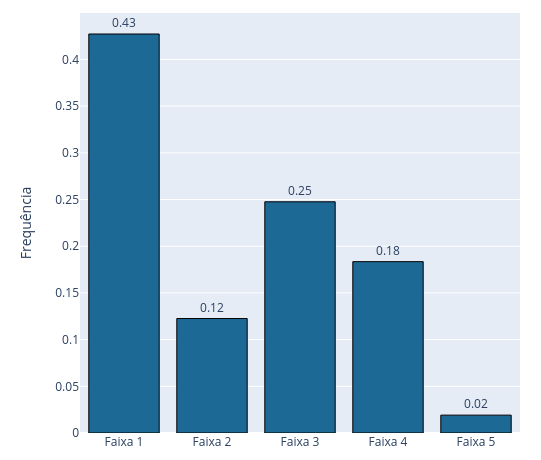
\includegraphics[scale= 0.5]{figuras/faixas_polymod-PIF.png}
        %PIF15102023
    %\captionsetup{font=small}
    \captionsetup{font=small,justification=justified}
    \caption*{Resultados da frequência de cada faixa etária no banco de dados POLYMOD, esse será um dos \textit{inputs} do modelo posteriormente.\\ Fonte: Autor.}

    \label{fig:freq}
\end{figure}

Com base nos dados obtidos, será realizada uma investigação para avaliar a duração, frequência e a presença de contato físico nos encontros em análise. A Figura \ref{fig:graficos} mostra os padrões dos contatos do POLYMOD; é possível ver que quanto mais frequente ou durável é o contato maior a chance dele ter contato físico.
Além disso, quanto mais frequente é o contato maiores as chances da conversa durar mais, por exemplo em contatos diários existe mais de 50\% de chance de que o contato dure mais que 1 hora. Por fim, o gráfico mais recente evidencia que, no ambiente domiciliar, a probabilidade de ocorrência de contato físico é significativamente maior, especialmente em áreas designadas para o lazer. Por contraste, no ambiente profissional, as chances são substancialmente menores, sendo considerado o cenário menos propenso a esse tipo de interação.

\begin{figure}[H]
    \centering
    \captionsetup{font=normalsize,skip=0.8pt,singlelinecheck=on,labelsep=endash}
    \caption{Probabilidade de contato físico}
    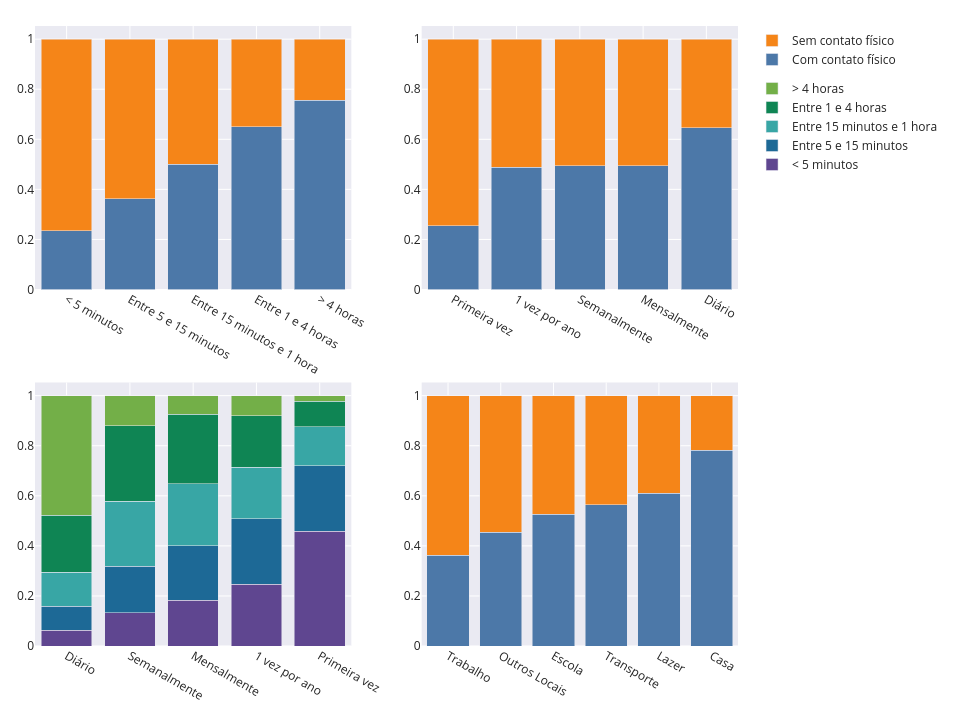
\includegraphics[scale= 0.45]{figuras/graficos-PIF.png}
\captionsetup{font=small,justification=justified}
    \caption*{Ilustra a relação entre a frequência e a duração dos contatos com a probabilidade de contato físico, mostrando que contatos mais frequentes e duradouros têm maior probabilidade de envolver contato físico. Além disso, o ambiente domiciliar apresenta maior probabilidade de contato físico, especialmente nas áreas de lazer, em comparação ao ambiente profissional, onde a probabilidade é consideravelmente menor. Todas as correlações são altamente significantes.\\ Fonte: Autor.}
    \label{fig:graficos}
\end{figure}


Um elemento importante que foi investigado foi como as idades influenciam nas conexões entre os indivíduos da rede. Na Figura \ref{fig:contatos_faixa} nota-se como é a distribuição de idades da pesquisa. Ao analisar a distribuição de ligações por faixa etária é percebido que seguem uma distribuição geométrica, que pode ser escrita como $P \propto (1 - p)^xp$ ou $P \propto e^{-\lambda x}(1 - e^\lambda)$. Na Figura \ref{fig:contatos_faixa} temos o estudo das distribuições como se fosse da segunda forma, no eixo das abscissas o grau e no eixo das ordenadas o logaritmo da probabilidade, com isso é encontrado uma reta com Mínimos Quadrados na qual o coeficiente angular é igual ao $\lambda$ e seu respectivo $R^2$. 

\begin{figure}[H]
    \centering
    \captionsetup{font=normalsize,skip=0.8pt,singlelinecheck=on,labelsep=endash}
    \caption{Influência das idades nas conexões}
    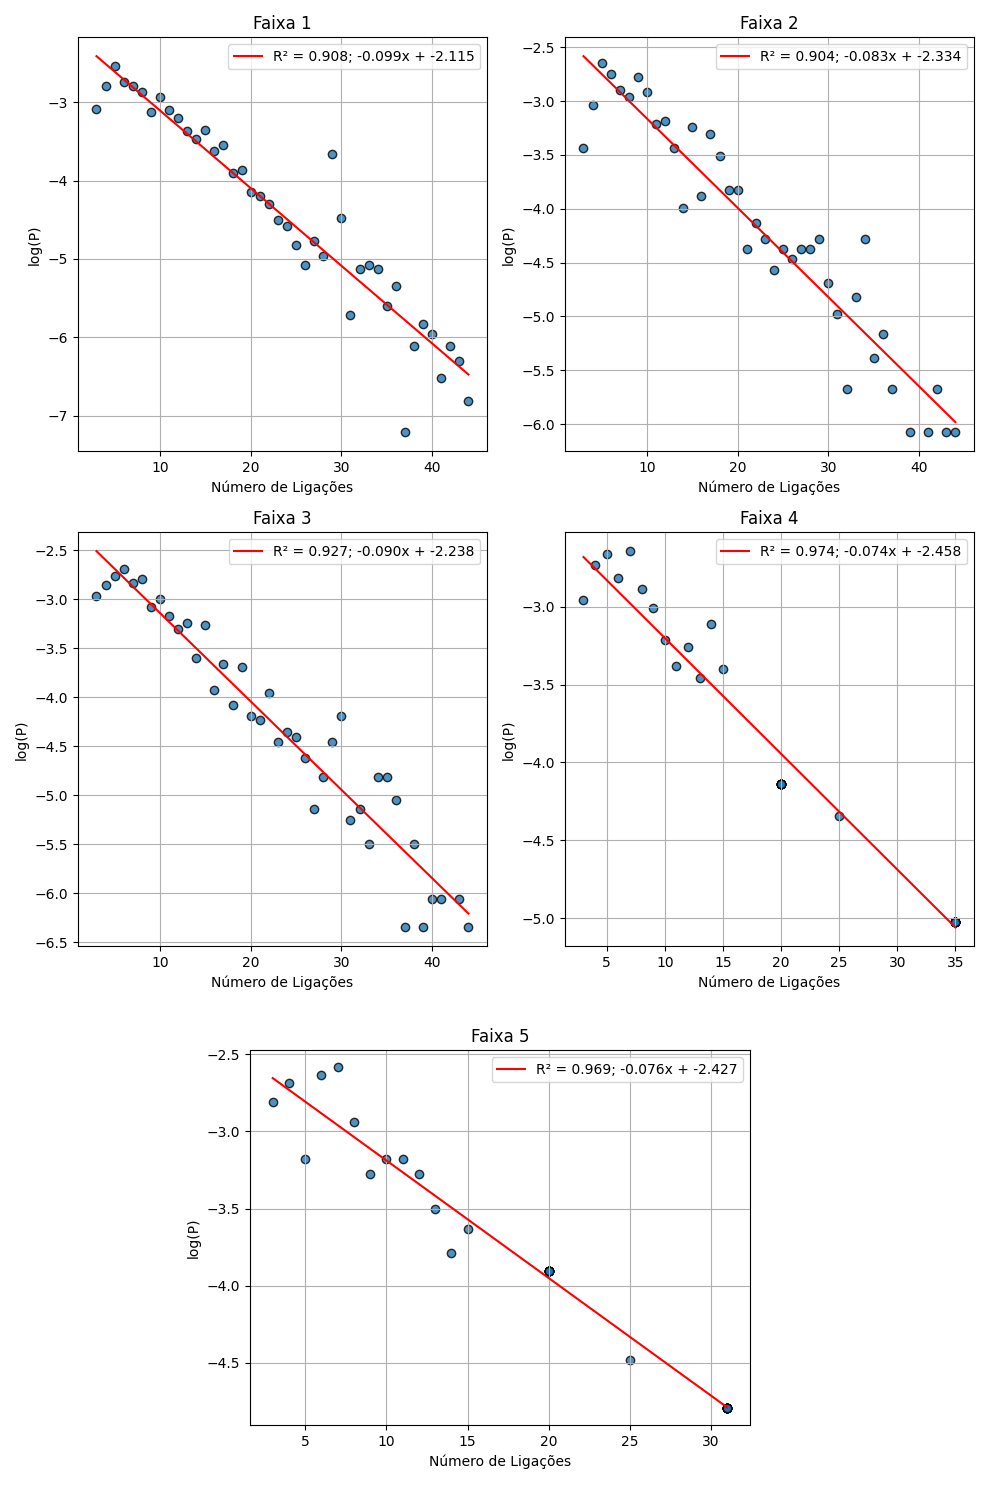
\includegraphics[scale= 0.3]{figuras/contatos_faixa.png}
    \captionsetup{font=small,justification=justified}
    \caption*{Ilustra a influência das idades nas 
    conexões da rede social, observando uma distribuição geométrica nas ligações por faixa etária.\\ Fonte: Autor.}
    \label{fig:contatos_faixa}
\end{figure}

A pesquisa também revela a relação entre a faixa etária de um indivíduo que preencheu o questionário e a distribuição de suas ligações. A Figura \ref{fig:heat} ilustra a frequência média de conexões para cada faixa etária. Observa-se um padrão consistente, independentemente da faixa etária; no entanto, os valores numéricos variam. Notavelmente, a faixa etária 3 apresenta a maior frequência de conexões, sendo composta majoritariamente por indivíduos que estão na fase produtiva da vida, muitas vezes já com família estabelecida. Em contraste, a última faixa etária demonstra a menor frequência de conexões, presumivelmente devido às dificuldades associadas a essa fase da vida.

\begin{figure}[H]
    \centering
    \captionsetup{font=normalsize,skip=0.8pt,singlelinecheck=on,labelsep=endash}
    \caption{Frequência média de conexões por faixa etária}
    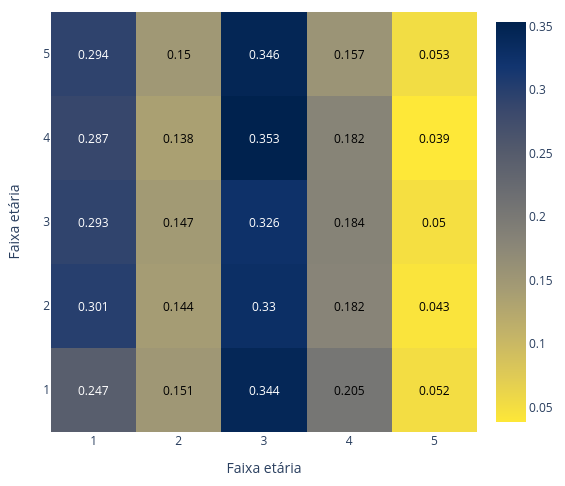
\includegraphics[scale= 0.5]{figuras/h-PIF.png}
    \captionsetup{font=small,justification=justified}
    \caption*{Mostra a frequência média de conexões por faixa etária, ressaltando que a faixa etária 3, associada à vida profissional e familiar, possui a maior frequência de conexões, enquanto a última faixa apresenta a menor frequência devido às dificuldades inerentes a essa fase da vida. \\Fonte: Autor}
    \label{fig:heat}
\end{figure}

Por último, a Figura \ref{fig:mediastd} apresenta duas matrizes de calor que ilustram a média e o desvio padrão do tempo de contato entre diferentes faixas etárias. A matriz da média mostra que as faixas etárias tendem a ter maior tempo de contato consigo mesmas e com faixas etárias adjacentes, com tempos decrescentes à medida que a diferença de idade aumenta. Notavelmente, a Faixa Etária 1 possui os maiores tempos médios de contato consigo mesma e com a Faixa Etária 2, enquanto os tempos são menores com as faixas etárias superiores e a Faixa Etária 4 apresenta contato elevado com a Faixa Etária 5.

\begin{figure}[H]
    \centering
    \captionsetup{font=normalsize,skip=0.8pt,singlelinecheck=on,labelsep=endash}
    \caption{Frequência média de conexões por faixa etária}
    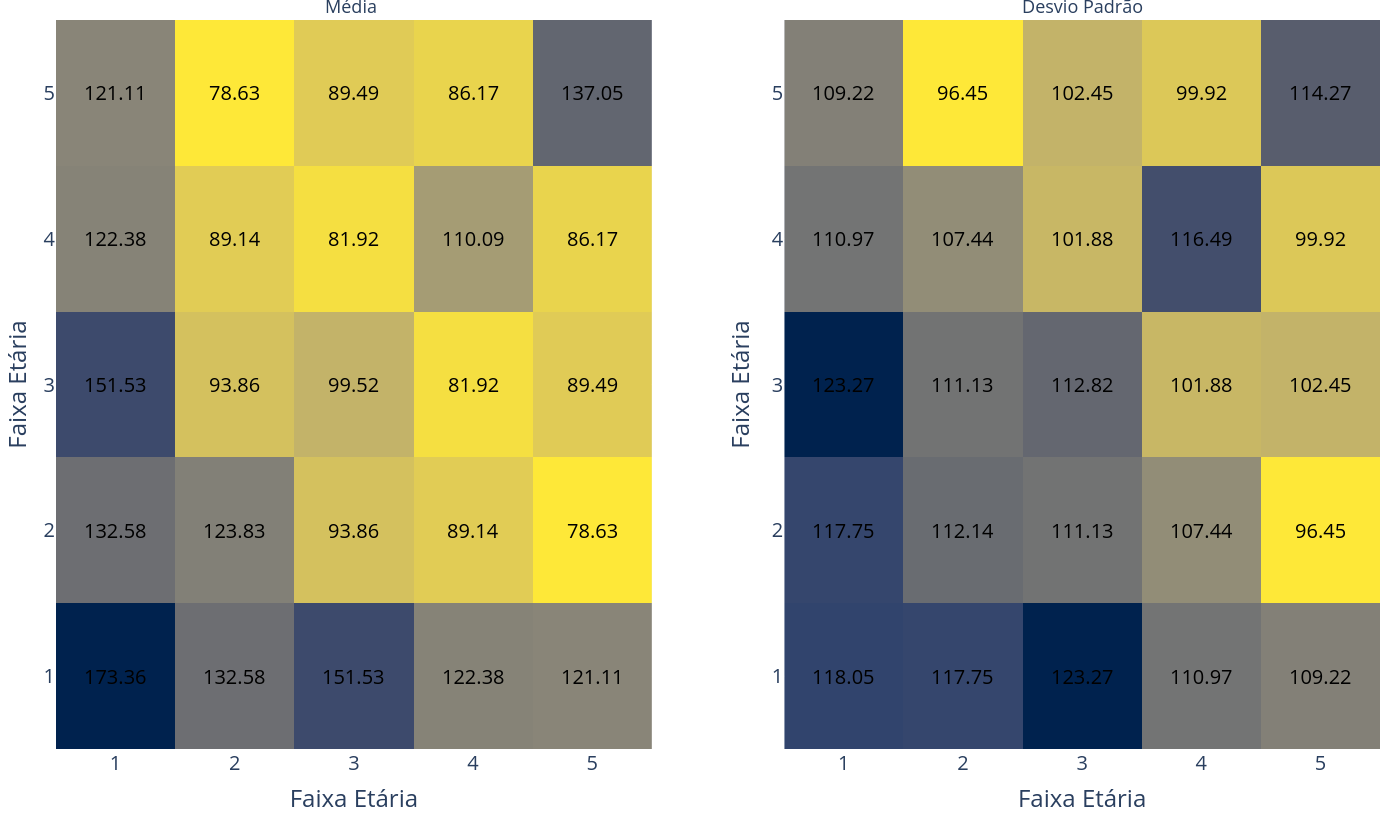
\includegraphics[scale= 0.35]{figuras/media_std.png}
    \captionsetup{font=small,justification=justified}
    \caption*{A imagem mostra a média e o desvio padrão do tempo de contato entre diferentes faixas etárias. A matriz da média indica que o contato é mais intenso dentro da mesma faixa etária e entre faixas etárias adjacentes, reduzindo conforme aumenta a diferença de idade. A matriz do desvio padrão mostra maior variação nos contatos dentro da mesma faixa e entre adjacentes, com menor variação entre faixas mais distantes. \\Fonte: Autor}
    \label{fig:mediastd}
\end{figure}

A matriz do desvio padrão indica que a variação no tempo de contato é mais significativa dentro da mesma faixa etária e com faixas etárias adjacentes, sugerindo maior inconstância nesses contatos. A Faixa Etária 1 apresenta o maior desvio padrão consigo mesma, seguido por desvios elevados com as Faixas Etárias 2 e 3, e menores com as Faixas Etárias 4 e 5. As Faixas Etárias 2 e 3 também exibem variações notáveis consigo mesmas e com faixas adjacentes, enquanto a Faixa Etária 4 tem maior variação com a Faixa Etária 5.

\subsection{Resultados da Rede gerada}

Os dados das Figuras 
\ref{fig:contatos_faixa} e \ref{fig:heat} serão utilizados como \textit{inputs} do Modelo de Configuração Ponderado, onde aquele vai ser usado para construir a distribuição empírica do grau de cada nó de cada faixa etária e este será usado como parâmetros de uma multinomial para estabelecer quantas ligações vão para cada faixa etária. A partir disso e dado um valor de $p$ 
(parâmetro que aumenta o coeficiente de agrupamento)
será construída a rede para acontecer a simulação da epidemia. As características dessa rede são mostradas na Tabela \ref{table:rrede} e na Figura \ref{fig:regressao}
mostra-se como evolui o agrupamento com o incremento de $p$, que cresce com $C \propto p^{\alpha}$, tanto o agrupamento médio quanto o total no qual $\alpha_{medio } = 0.46$ e $\alpha_{medio } = 0.55$. Após a aplicação do algoritmo foi recolhido os dados da rede e observou-se que para qualquer valor de $p$ a distribuição de graus tinha a mesma distribuição que a encontrada pela Figura \ref{fig:contatos_faixa} a partir do teste de Kolmogorov-Smirnov (Figura \ref{fig:comparacao}) \cite{manual} e na Tabela \ref{tab:pvalor} mostra a lista dos P-valores para cada valor de $p$. Na Figura \ref{fig:modelo}
mostra-se a diferença absoluta ao final do algoritmo da proporção de conexões de cada faixa etária em comparação com a Figura \ref{fig:heat}, tendo uma diferença maior entre as conexões com faixa etária 1.


\begin{table}[H]
    \centering
    \captionsetup{font=normalsize,skip=0.8pt,singlelinecheck=on,labelsep=endash}
    \caption{P-valores para diferentes valores de $p$.}
    \begin{tabular}{|c|c|c|c|c|c|}
    
    \hline
    \multirow{2}{*}{$p$} & \multicolumn{5}{c|}{Faixa Etária} \\ \cline{2-6} 
     & 1 & 2 & 3 & 4 & 5 \\ \hline
    0 & 1.0 & 0.992 & 0.975 & 0.851 & 0.434 \\ \hline
    \rowcolor{Gray}
    0.5 & 1.0 & 0.903 & 1.0 & 0.092 & 0.146 \\ \hline
    1.0 & 1.0 & 0.988 & 1.0 & 0.772 & 0.993 \\ \hline
    \end{tabular}
    \label{tab:pvalor}
\end{table}

\begin{figure}[H]
    \centering
    %PIF27092023
    \captionsetup{font=normalsize,skip=0.8pt,singlelinecheck=on,labelsep=endash}
    \caption{Agrupamento da rede em função de $p$}
    %PIF27092023 É possível apagar o enquadramento branco?        
    %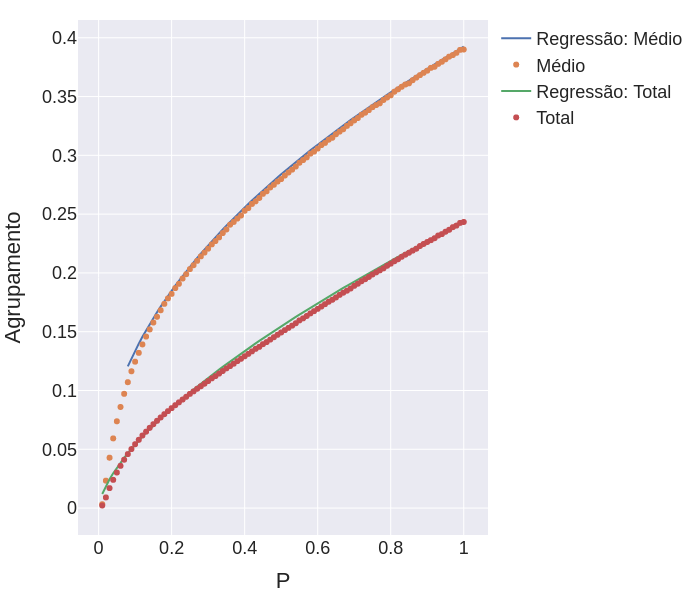
\includegraphics[scale= 0.5]{figuras/clustering_vs_p.png}
    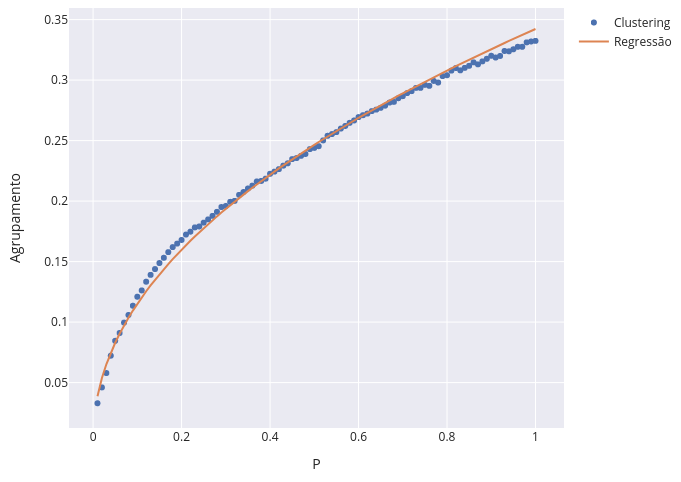
\includegraphics[scale= 0.5]{figuras/clustering_vs_p-PIF.png}
    %PIF27092023
    %\caption{Evolução do agrupamento da rede em função 
    %PIF15102023
    %\captionsetup{font=small}
    \captionsetup{font=small,justification=justified}    \caption*{Evolução do agrupamento da rede em função 
    do incremento do valor de $p$, foi utilizada uma regressão linear para saber qual a função que rege encontrando $C \propto p^{\alpha}$.\\Fonte: Autor}
    \label{fig:regressao}
\end{figure}


\begin{figure}[H]
    \centering
    
    \captionsetup{font=normalsize,skip=0.8pt,singlelinecheck=on,labelsep=endash}
    \caption{Resultados da proporção de conexões entre faixas}
    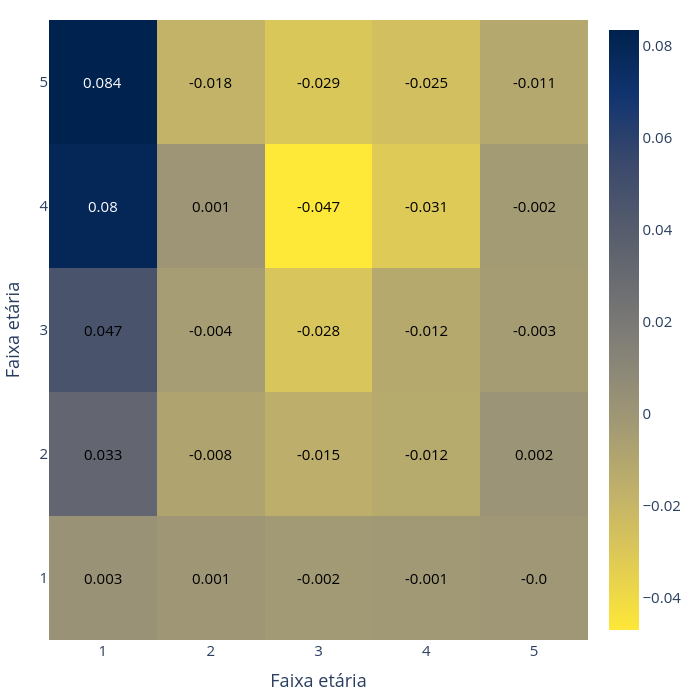
\includegraphics[scale= 0.4]{figuras/modelo.png}
        %PIF15102023
    %\captionsetup{font=small}
    \captionsetup{font=small,justification=justified}
    \caption*{ A figura mostra a diferença absoluta entre a matriz de proporções de conexões entre as faixas etárias do modelo e do encontrado no POLYMOD essa diferença se mantém constante independe do valor de $p$.}
    \label{fig:modelo}
\end{figure}


\begin{table}[H]

  %PIF15102023
%  \centering
%  \captionsetup{margin={9pt,14pt},font=normalsize,skip=0.5pt,labelsep=endash}
\captionsetup{font=normalsize,skip=0.8pt,singlelinecheck=on,labelsep=endash}
\caption{Métricas das redes geradas.}
  \centering
  \hspace*{-\leftmargin}\begin{tabular}{lcccccc}

    \hline

    \multicolumn{1}{l|}{ \textbf{\shortstack{$p$}}} & 
    \multicolumn{1}{c|}{\textbf{\shortstack{Grau \\ Médio}}}  & 
    \multicolumn{1}{c|}{\textbf{\shortstack{Grau \\ Mediano}}} &
    \multicolumn{1}{c|}{\textbf{\shortstack{Desvio \\ Padrão \\ Grau}}} &
    \multicolumn{1}{c|}{\textbf{\shortstack{Agrupa-\\mento \\ Médio}}} & 
    \multicolumn{1}{c|}{\textbf{\shortstack{Menor \\ Caminho \\ Médio}}} & 
    \multicolumn{1}{c}{{\shortstack{\textbf{Diâmetro}}}}     \\

    \hline
    
    0 & 13.24(0.23) & 10.024(0.19) & 10.38(0.22) & 0.01(0.00) & 3.26(0.02) & 6.778(0.48) \\
    \rowcolor{Gray}
    0.5 & 13.27(0.22) & 10.037(0.21) & 10.39(0.22) & 0.21(0.01) & 3.39(0.02) & 7.123(0.41) \\
    
    1.0 & 13.27(0.22) & 10.034(0.22) & 10.40(0.22) & 0.31(0.01) & 3.51(0.03) & 7.333(0.54) \\
    \hline

    
\end{tabular}

\caption*{Com o incremento de $p$ houve um aumento significativo no agrupamento, como esperado, o que acarretou em um aumento do menor caminho médio e do diâmetro da rede.}
\label{table:rrede}
\end{table}

\begin{figure}[H]
    \centering
    \captionsetup{font=normalsize,skip=0.8pt,singlelinecheck=on,labelsep=endash}
    \caption{Distribuição de Graus $p = 1.0$}
    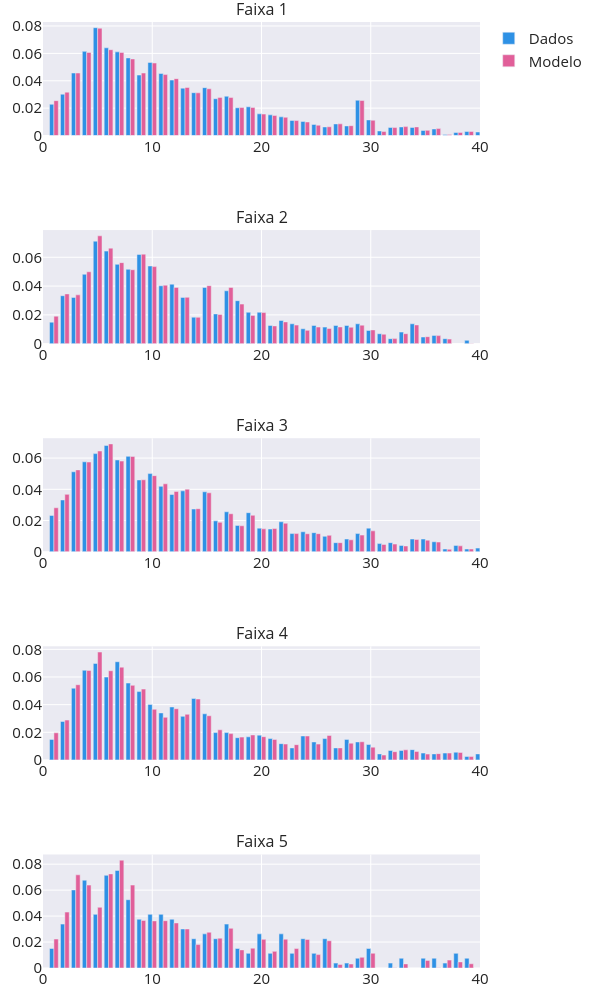
\includegraphics[scale= 0.4]{figuras/comparacao.png}
    \captionsetup{font=small,justification=justified}
    \caption*{Comparação de como fica a distribuição de graus comparando modelo com $p = 1.0$ com dados do POLYMOD, é possível ver que a Faixa etária 4 e 5 são as mais afetadas mas apresentam a mesma distribuição de acordo com o Teste.\\Fonte: Autor}
    \label{fig:comparacao}
\end{figure}

Texto texto texto texto texto texto texto texto texto texto texto texto texto texto texto texto texto texto texto texto texto texto texto texto texto texto texto texto texto texto texto texto texto texto texto texto texto texto texto texto texto texto texto texto texto texto texto texto texto texto texto texto texto texto texto texto texto texto texto texto texto texto texto texto texto texto texto texto texto.

\section{Resultados do Experimento A}
\label{sec:resultados-do-experimento-a}

Procure deixar as figuras dos resultados o maior possível preenchendo a largura do texto do documento que possui $16~cm$.

\begin{figure}[H]
        \captionsetup{width=16cm}
		\Caption{\label{fig:tensaoimpedanciahumana} Gráfico de tensão considerando a impedância humana}
		%\centering
		\UFCfig{}{
			\fbox{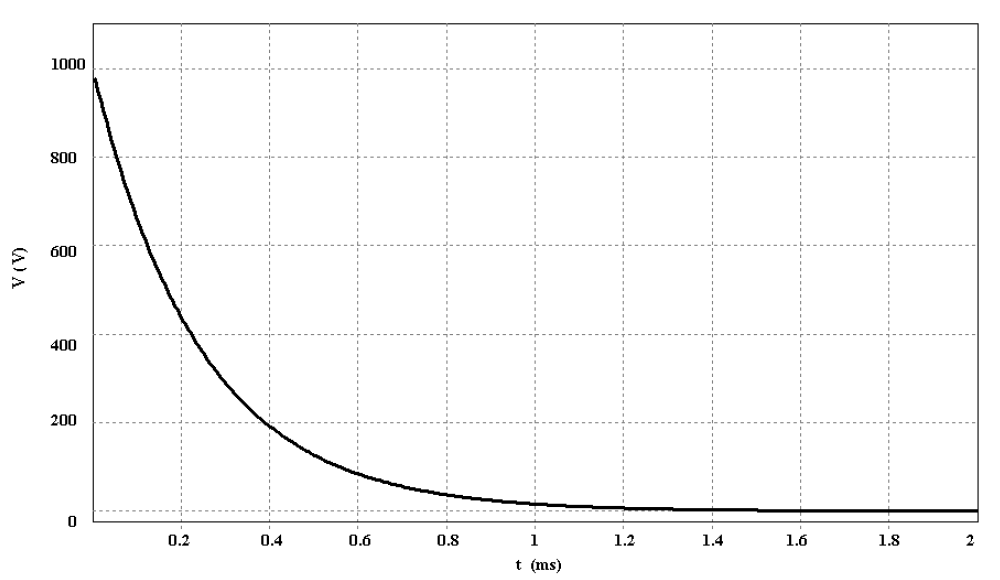
\includegraphics[width=16cm]{figuras/tensaoimpedanciahumana}}
		}
			\Fonte{elaborada pelo autor.}
			
\end{figure}

Texto texto texto texto texto texto texto texto texto texto texto texto texto texto texto texto texto texto texto texto texto texto texto texto texto texto texto texto texto texto texto texto texto texto texto texto texto texto texto texto texto texto texto texto texto texto texto texto texto texto texto texto texto texto texto texto texto texto texto texto texto texto texto texto texto texto texto texto texto.

\begin{figure}[h!]
	\captionsetup{width=16cm}
	\Caption{\label{fig-grafico-1}Produção anual das dissertações de mestrado e teses de doutorado entre os anos de 1990 e 2008}		
	\IBGEtab{}{
		\fbox{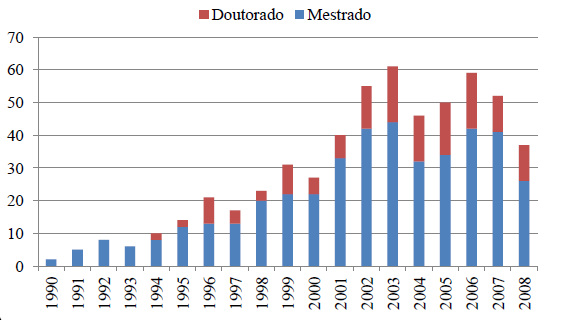
\includegraphics[width=16cm]{figuras/figura-3}}
	}{
	\Fonte{elaborada pelo autor.}
}
\end{figure}

Texto texto texto texto texto texto texto texto texto texto texto texto texto texto.

Texto texto texto texto texto texto texto texto texto texto texto texto texto texto texto texto texto texto texto texto texto texto texto texto texto texto texto texto texto texto texto texto texto texto texto texto texto texto texto texto texto texto texto texto texto texto texto texto texto texto texto texto texto texto texto texto texto texto texto texto texto texto texto texto texto texto texto texto texto.

\section{Resultados do Experimento B}
\label{sec:resultados-do-experimento-b}

Referenciando a \autoref{tab:notas}. Texto texto texto texto texto texto texto texto texto texto texto texto texto texto texto texto texto texto texto texto texto texto texto texto texto texto texto texto texto texto texto texto.

\begin{table}[!ht]	
	%\centering
	\captionsetup{width=11.3cm}%ATENÇÃO: Ajuste a largura do título
	\Caption{\label{tab:notas} Notas dos participantes nas avaliações A, B e C}	
	\IBGEtab{}{
		\begin{tabular}{crrr}
			\toprule
			Identificação dos participantes & Avaliação A & Avaliação B &                        Avaliação C \\
			\midrule \midrule
			Participante 1 & 7 & 9 & 10\\
			Participante 2 & 8 & 2 & 1\\
			Participante 3 & 5 & 10 & 6 \\
			Participante 4 & 3 & 1 & 4\\
			Participante 5 & 2 & 4 & 1\\
			Participante 6 & 0 & 7 & 2\\
			\bottomrule
		\end{tabular}
	}{
	\Fonte{elaborada pelo autor.}
}
\end{table}

Texto texto texto texto texto texto texto texto texto texto texto texto texto texto texto texto texto texto texto texto texto texto texto texto texto texto texto texto texto texto texto texto texto texto texto texto texto texto texto texto texto texto texto texto texto texto texto texto texto texto texto texto texto texto texto texto texto texto texto texto texto texto texto texto texto texto texto texto texto.Texto texto texto texto texto texto texto texto texto texto texto texto texto texto texto texto texto texto texto texto texto texto texto texto texto texto texto texto texto texto texto texto texto texto texto texto texto texto texto texto texto.

Texto texto texto texto texto texto texto texto texto texto texto texto texto texto texto texto texto texto texto texto texto texto texto texto texto texto texto texto texto texto texto texto texto texto texto texto texto texto texto texto texto texto texto texto texto texto texto texto.Texto texto texto texto texto texto texto texto texto texto texto texto texto texto texto texto texto texto texto texto texto.

Referenciando a \autoref{tab:notas}. Texto texto texto texto texto texto texto texto texto texto texto texto texto texto texto texto texto texto texto texto texto texto texto texto texto texto texto texto texto texto texto texto texto texto texto texto texto texto texto texto texto texto texto texto texto texto texto texto texto texto texto texto texto texto texto texto texto texto texto texto texto texto texto texto texto texto texto.